\documentclass[tikz,border=2mm]{standalone}
\usetikzlibrary{arrows.meta,calc,decorations.pathreplacing,positioning}

\definecolor{manifoldFill}{RGB}{229,241,255}
\definecolor{manifoldDraw}{RGB}{57,98,150}
\definecolor{groupFill}{RGB}{236,248,236}
\definecolor{groupDraw}{RGB}{58,122,69}
\definecolor{flowRed}{RGB}{190,55,48}
\definecolor{actionPurple}{RGB}{105,77,168}
\definecolor{textGray}{RGB}{70,70,70}

\begin{document}
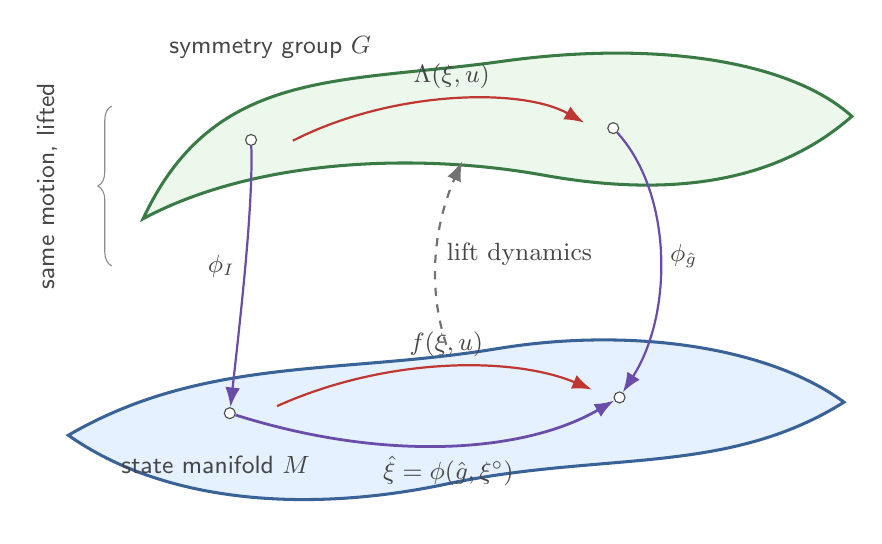
\begin{tikzpicture}[
  >=Latex,
  font=\sffamily,
  label/.style={font=\small\sffamily, text=textGray},
  mathlabel/.style={font=\small, text=textGray},
  state/.style={circle, draw=black!70, fill=white, inner sep=1.4pt},
  arrow/.style={line width=0.8pt, -{Latex[length=2.5mm]}},
  flow/.style={arrow, draw=flowRed},
  action/.style={arrow, draw=actionPurple},
  lift/.style={arrow, draw=black!55, dashed}
]

% The state manifold.
\path[fill=manifoldFill, draw=manifoldDraw, line width=1.1pt]
  (-4.9,-1.20)
  .. controls (-3.7,-2.05) and (-1.9,-2.20) .. (-0.1,-1.82)
  .. controls (1.9,-1.40) and (3.45,-1.72) .. (4.95,-0.78)
  .. controls (4.0,-0.08) and (2.25,0.18) .. (0.55,-0.10)
  .. controls (-1.45,-0.43) and (-3.18,-0.20) .. (-4.9,-1.20)
  -- cycle;
\node[label, anchor=west] at (-4.35,-1.58) {state manifold $M$};

% Manifold points and dynamics.
\node[state, label={[mathlabel]below:$\xi^\circ$}] (xref) at (-2.85,-0.92) {};
\node[state, label={[mathlabel]below:$\hat{\xi}$}] (xhat) at (2.10,-0.72) {};
\draw[flow] (-2.25,-0.83)
  .. controls (-0.85,-0.20) and (0.75,-0.20) .. (1.75,-0.62)
  node[midway, above, mathlabel] {$f(\xi,u)$};
\draw[action, line width=1.0pt] (xref)
  .. controls (-0.85,-1.55) and (0.90,-1.42) .. (xhat)
  node[midway, below, mathlabel] {$\hat{\xi}=\phi(\hat{g},\xi^\circ)$};

% The hovering symmetry group.
\path[fill=groupFill, draw=groupDraw, line width=1.1pt]
  (-3.95,1.55)
  .. controls (-2.55,2.30) and (-0.50,2.40) .. (1.15,2.10)
  .. controls (2.95,1.78) and (4.20,2.10) .. (5.05,2.85)
  .. controls (4.28,3.55) and (2.58,3.82) .. (0.62,3.55)
  .. controls (-1.45,3.26) and (-3.05,3.48) .. (-3.95,1.55)
  -- cycle;
\node[label, anchor=west] at (-3.74,3.72) {symmetry group $G$};

% Group points and lifted dynamics.
\node[state, label={[mathlabel]above:$I$}] (gid) at (-2.58,2.55) {};
\node[state, label={[mathlabel]above:$\hat{g}$}] (ghat) at (2.02,2.70) {};
\draw[flow] (-2.05,2.54)
  .. controls (-0.80,3.18) and (0.85,3.22) .. (1.65,2.77)
  node[midway, above, mathlabel] {$\Lambda(\xi,u)$};

% Lift and action relationships.
\draw[lift] (-0.10,-0.05)
  .. controls (-0.35,0.70) and (-0.25,1.48) .. (0.10,2.28)
  node[midway, right, mathlabel] {lift dynamics};

\draw[action] (ghat)
  .. controls (2.78,1.86) and (2.78,0.34) .. (xhat)
  node[midway, right, mathlabel] {$\phi_{\hat{g}}$};
\draw[action] (gid)
  .. controls (-2.55,1.72) and (-2.72,0.25) .. (xref)
  node[midway, left, mathlabel] {$\phi_I$};

% Explanatory brace.
\draw[decorate, decoration={brace, amplitude=5pt}, draw=black!45]
  (-4.35,0.95) -- (-4.35,2.98)
  node[midway, xshift=-0.82cm, rotate=90, label] {same motion, lifted};

\end{tikzpicture}
\end{document}
